\hypertarget{querschnittliche-konzepte}{%
\section{Querschnittliche Konzepte}\label{querschnittliche-konzepte}}

\textbf{Inhalt}

Dieser Abschnitt beschreibt übergreifende, prinzipielle Regelungen und
Lösungsansätze, die an mehreren Stellen (=\emph{querschittlich})
relevant sind.

Solche Konzepte betreffen oft mehrere Bausteine. Dazu können vielerlei
Themen gehören, beispielsweise:

\begin{itemize}
\tightlist
\item
  fachliche Modelle,
\item
  eingesetzte Architektur- oder Entwurfsmuster,
\item
  Regeln für den konkreten Einsatz von Technologien,
\item
  prinzipielle --- meist technische --- Festlegungen übergreifender Art,
\item
  Implementierungsregeln
\end{itemize}

\textbf{Motivation}

Konzepte bilden die Grundlage für \emph{konzeptionelle Integrität}
(Konsistenz, Homogenität) der Architektur und damit eine wesentliche
Grundlage für die innere Qualität Ihrer Systeme.

Manche dieser Themen lassen sich nur schwer als Baustein in der
Architektur unterbringen (z.B. das Thema „Sicherheit"). Hier ist der
Platz im Template, wo Sie derartige Themen geschlossen behandeln können.

\textbf{Form}

Kann vielfältig sein:

\begin{itemize}
\item
  Konzeptpapiere mit beliebiger Gliederung,
\item
  übergreifende Modelle/Szenarien mit Notationen, die Sie auch in den
  Architektursichten nutzen,
\item
  beispielhafte Implementierung speziell für technische Konzepte,
\item
  Verweise auf „übliche" Nutzung von Standard-Frameworks (beispielsweise
  die Nutzung von Hibernate als Object/Relational Mapper).
\end{itemize}

\textbf{Struktur}

Eine mögliche (nicht aber notwendige!) Untergliederung dieses
Abschnittes könnte wie folgt aussehen (wobei die Zuordnung von Themen zu
den Gruppen nicht immer eindeutig ist):

\begin{itemize}
\tightlist
\item
  Fachliche Konzepte
\item
  User Experience (UX)
\item
  Sicherheitskonzepte (Safety und Security)
\item
  Architektur- und Entwurfsmuster
\item
  Unter-der-Haube
\item
  Entwicklungskonzepte
\item
  Betriebskonzepte
\end{itemize}

\begin{figure}
\centering
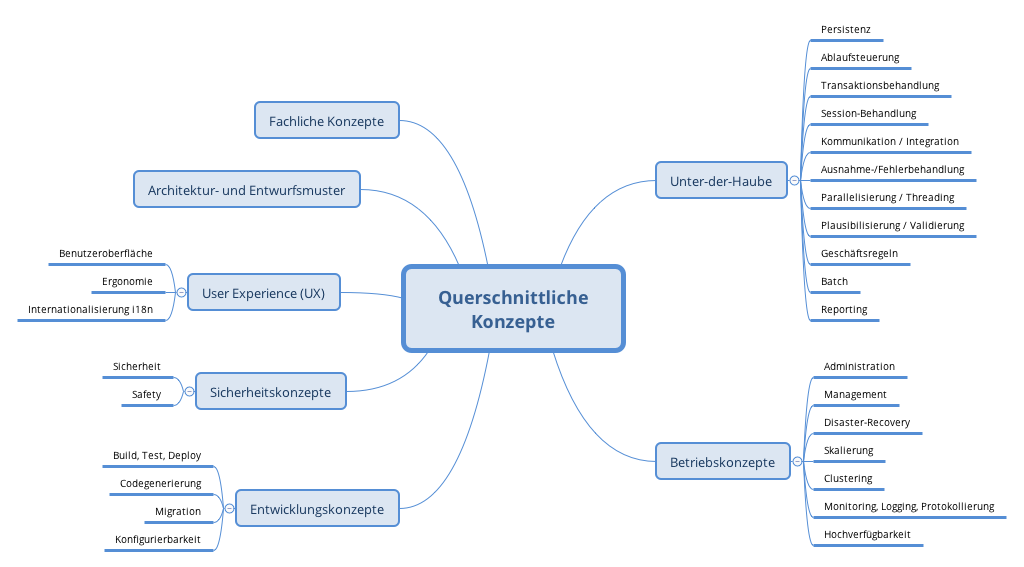
\includegraphics{../images/08-Crosscutting-Concepts-Structure-DE.png}
\caption{Possible topics for crosscutting concepts}
\end{figure}

\hypertarget{konzept-1}{%
\subsection{\texorpdfstring{\emph{\textless Konzept
1\textgreater{}}}{\textless Konzept 1\textgreater{}}}\label{konzept-1}}

\emph{\textless Erklärung\textgreater{}}

\hypertarget{konzept-2}{%
\subsection{\texorpdfstring{\emph{\textless Konzept
2\textgreater{}}}{\textless Konzept 2\textgreater{}}}\label{konzept-2}}

\emph{\textless Erklärung\textgreater{}}

\ldots{}

\hypertarget{konzept-n}{%
\subsection{\texorpdfstring{\emph{\textless Konzept
n\textgreater{}}}{\textless Konzept n\textgreater{}}}\label{konzept-n}}

\emph{\textless Erklärung\textgreater{}}
